%\chapterauthor{Second Author}{Second Author Affiliation}
\chapter{Quantum Field Theory}
\chapterauthor{Ivo Iliev\\Sofia University}
\adjustmtc
\minitoc

\section{Rarita-Schwinger equation}
Consider the following Lagrangian
\begin{equation}
  \mathcal{L} = -\frac{1}{2}\bar{\psi}_\mu\left(\epsilon^{\mu\kappa\rho\nu}\gamma_5\gamma_\kappa\partial_\rho-im\sigma^{\mu\nu}\right)\psi_\nu
\end{equation}
This equation obviously controls the propagation of the wave function of
a spin- object such as the gravitino. The equation of motion for
this Lagrangian are known as the \textit{Rarita-Schwinger equation}:
\begin{equation}
\left(\epsilon^{\mu\kappa\rho\nu}\gamma_5\gamma_\kappa\partial_\rho
  -im\sigma^{\mu\nu}\right)\psi_\nu
\end{equation}
In the massless case, the Rarita-Schwinger equation has a fermionic gauge
symmetry, it is invariant under the gauge transformation:
\begin{equation}
  \psi_\mu\rightarrow\psi_\mu + \partial_\mu\epsilon,
\end{equation}
where $\epsilon\equiv\epsilon_\alpha$ is an arbitrary spinor field. 
\subsection{Massless case}
Consider a massless Rarita-Schwinger field, described by the Lagrangian
\begin{equation}
  \mathcal{L}_{RS} = \bar{\psi}_\mu\gamma^{\mu\nu\rho}\partial_\nu\psi_{\rho}
\end{equation}
where the sum over spin indices is implicit, $\psi_\mu$ are Majorana spinors
and the quantity $\gamma^{\mu\nu\rho}$ is equal to
\begin{equation}
  \gamma^{\mu\nu\rho}\equiv\frac{1}{3!}\gamma^{[\mu}\gamma^\nu\gamma^{\rho]}
\end{equation}
Varying the Lagrangian yields after some calculation
\begin{equation}
  \delta\mathcal{L_{RS}}
  = 2\delta\bar{\psi}_\mu\gamma^{\mu\nu\rho}\partial_\nu\psi_\rho
  + \text{boundary terms}
\end{equation}
Now imposing that $\mathcal{L}_{RS} =0$ we get the equation of motion for
a massless Majorana Rarita-Schwinger spinor:
\begin{equation}
  \gamma^{\mu\nu\rho}\partial_\nu\psi_\rho = 0
\end{equation}
\subsection{Massive case}
The description of massive, higher-spin fields through the Rarita-Schwinger
equation is not well defined physically. Coupling the RS Largrangian to
electromagnetism leads to an equation with solutions representing wavefronts,
some of which propagate faster than light. However, it was shown by Das and
Freedman that local supersymmetry can circumvent this problem.



\section{Wilson Loops and Large N}
This section is dedicated to a short introduction to the methods used in
nonperturbative investigations of QCD and other gauge theories. The main
attention is payed to Wilson loops, both on the lattice and in the continuum,
which play a central role in modern formulations of gauge theories and to the
method of the large $N$ expansion.

\subsection{Wilson Loops}
In essence, Wilson loops are phase factors in Abelian or non-Abelian gauge
theories. Wilson loops are observable in quantum theory by the Aharonov-Bohm
effect. Wilson loops play a central role in the lattice formulation of gauge
theories. QCD can be reformulated through Wilson loops in a manifest
gauge-invariant way. Analogues of the Wilson loops are extremely useful in
solving various kinds of matrix models.
\subsubsection{Phase factors in QED}
\par Let us first examine the familiar setting of QED. An Abelian phase factor
is defined by the formula
\begin{equation}
  U\left[\Gamma_{yx}\right] = e^{ie\int_{\Gamma_{yx}\mathrm{d}z^\mu
  A_\mu(z)}}
  \label{eq:abelianphasefactor}
\end{equation}

Under the gauge transformation this becomes

\begin{equation}
  A_\mu(z)\xrightarrow{\text{g.t.}} A_\mu(z)+ \frac{1}{e}\partial_\mu\alpha(z)
\end{equation}
and the Abelian phase factor transforms as 
\begin{equation}
  U\left[\Gamma_{yx}\right]\xrightarrow{\text{g.t.}}
  \mathrm{e}^{i\alpha{y}}  U\left[\Gamma_{yx}\right]
  \mathrm{e}^{-i\alpha{x}}
\end{equation}
It is easy to show that a wave function at the point $x$ is transformed as
\begin{equation}
  \phi(x)\xrightarrow{\text{g.t.}}\mathrm{e}^{i\alpha(x)}\psi(x),
\end{equation}
therefore the phase factor is transformed as the product
$\psi(y)\psi^\dagger(x)$:
\begin{equation}
  U\left[\Gamma_{yx}\right]\stackrel{g.t.}{\sim} "\psi(y)\psi^\dagger(x)"
\end{equation}
  A wave function at the point $x$ transforms like one at the point $y$ after
  multiplication by a phase factor:
\begin{equation}
    U\left[\Gamma_{yx}\right]\psi(x)\stackrel{g.t.}{\sim} "\psi(y)",
\end{equation}
and analogously
\begin{equation}
  \psi^\dagger(y) U\left[\Gamma_{yx}\right] \stackrel{g.t.}{\sim}
  "\psi^\dagger(x)".
\end{equation}
The phase factor plays the role of a parallel transporter in an electromagnetic
field, and to compare phases of a wave function at points $x$ and $y$, we
should first make a parallel transport along some contour $\Gamma_{yx}$. The
result is of course $\Gamma$-dependent except when $A_\mu(z)$ is a pure gauge
(meaning that the field strength $F_{\mu\nu}(z)$ is vanishing along the
contour). Certain subtleties occur for not simply connected spaces, namely the
Aharonov-Bohm effect. 

\subsubsection{Propagators in external field}
Let us consider a quantum particle in a classical electromagnetic field. To
introduce electromagnetism field, $\partial_\mu$ is to be replaced by the
covariant derivative
\begin{equation}
  \partial_\mu \rightarrow \Delta_\mu = \partial_\mu - ieA_\mu(x).
\end{equation}
For the propagator we get
\begin{equation}
  G(x,y;A) = \frac{1}{2}\int_0^\infty\mathrm{d}\tau e^{-\frac{1}{2}\tau
      m^2}\int\limits_{\substack{z_\mu(0)=x_\mu\\ z_\mu(\tau)=y_\mu
        }}{\mathcal{D}z_\mu(t)e^{-\frac{1}{2}\int_0^\tau
        \mathrm{d}t\dot{z}^2_\mu(t)
    + ie\int_0^\tau\mathrm{d}t\dot{z}^\mu(t)A_\mu(z(t))}}
\end{equation}
Although this may seem cumbersome, one can easily spot that the exponent is
just the classical (Eucleadian) \textit{action} of a particle in an
external electromagnetic field. The path integral representation above for the
propagator of a scalar particle is due to Feynman. We can alternatively rewrite
it in a more compact form
\begin{equation}
  G(x,y;A)
  = \sum_{\Gamma_{yx}}{e^{S_{\mathrm{free}}[\Gamma_{yx}]+ie\int_{\Gamma_{yx}}\mathrm{d}z^\mu
  A_\mu(z)}},
\end{equation}
where we represented the (parametric invariant) integral over $\mathrm{d}t$ as
the contour integral along the trajectory $\Gamma_{yx}$ over
\begin{equation}
  \mathrm{d}z^\mu = \mathrm{d}t \dot{z}^\mu(t).
\end{equation}

The transition amplitude of a quantum particle in a classical electromagnetic
field is the sum over paths of the Abelian phase
factor\eqref{eq:abelianphasefactor}.

\subsubsection{Aharonov-Bohm effect}
\begin{figure}
  \label{fig:aharonov}
  \centering
  \caption{Aharonov-Bohm effect}
\end{figure}
Transverse components of the  electromagnetic field describe photons.
Longitudal components are related to gauging the phase of a wave function, i.e.
permit one to compare its values at different space-time points when an
electron is placed in an external electromagnetic field.
\par In quantum mechanics, the wave-function phase itself is not observable.
Only the phase differences are observable, e.g. via interference phenomena. The
phase difference depends on the value of the phase factor for a  given path
$\Gamma_{yx}$ along which the parallel transport is performed.
\par The phase factors are observable in quantum theory, in contrast to
classical theory. This is seen in the Aharonov-Bohm effect, whose scheme is
depicted in Fig. \ref{fig:aharonov}. Electrons do not pass inside the solenoid
where the magnetic field is concentrated. Nevertheless, a phase difference
arises between the electron beams passing through the two slits. The
interference picture changes with the value of the electric current.
The phase difference depends on (the real part of)
\begin{equation}
e^{ie\int_{\Gamma^+_{yx}}\mathrm{d}z^\mu A_\mu(z)}
e^{-ie\int_{\Gamma^-_{yx}}\mathrm{d}z^\mu A_\mu(z)}
  = e^{ie\oint_\Gamma\mathrm{d}z^\mu A_\mu(z)}
  = e^{ie\int\mathrm{d}\sigma^{\mu\nu}F_{\mu\nu}} = e^{ieHS}
\end{equation}
where the contour $\Gamma$ is composed from $\Gamma^+_{yx}$ and
$\Gamma^-_{xy}$. It does not depend on the shape of the two sub-contours but
depends only on $HS$ - the magnetic flux through the solenoid.
\subsection{Yang-Mills Theories}
Modern theories of fundamental particles are gauge theories. The principle of
local gauge invariance was introduced by H.Weyl for the electromagnetic
interaction in analogy with general covariance in Einstein's theory of
gravitation. An extension to non-Abelian gauge groups was given by Yang and
Mills in 1954.
\par A crucial role in gauge theories is played by the phase factor which is
associated with parallel transport in an external gauge field. The phase
factors are observable in quantum theory, in contrast to classical theory. This
is analogous to the  Aharonov-Bohm effect for the electromagnetic field.

\subsubsection{Gauge invariance}
The principle of local gauge invariance deals with the gauge transformation of
a matter field $\psi$, which is given by:

\begin{equation}
  \psi(x)\xrightarrow{g.t.}\psi'(t) = \Omega(x)\psi(x).
  \label{eq:gaugetransform}
\end{equation}

Here $\Omega(x)\in G$ with $G$ being a semisimple Lie group which is called the
gauge group $(G=SU(3)$ for QCD. \eqref{eq:gaugetransform} demonstrates
that $\psi$ belongs to the fundamental representation of $G$.
\par The unitary gauge group is when
\begin{equation}
  \Omega^{-1}(x) = \Omega^\dagger(x),
\end{equation}
while an extension to the other Lie groups is straightforward. 
Then we have

\begin{equation}
  \psi^\dagger(x) \xrightarrow{g.t.} \psi^{'\dagger}
  = \psi^\dagger(x)\Omega^\dagger(x).
\end{equation}
In analogy with QCD, the gauge group $G=SU(N)$ is usually associated with color
and the proper index of $\psi$ is called the color index.
\par The gauge transformation \eqref{eq:gaugetransform} of the matter field
$\psi$ can be compensated by a transformation of the non-Abelian gauge field
$\mathcal{A}_\mu$ which belongs to the adjoint representation of G:

\begin{equation}
  \mathcal{A}_\mu(x)\xrightarrow{g.t.}\mathcal{A}_\mu'(x)
  = \Omega(x)\mathcal{A}_\mu(x)\Omega^\dagger(x)
  + i\Omega(x)\partial_\mu\Omega^\dagger(x)
  \label{eq:nonabeliangaugetransform}
\end{equation}

It is convenient to introduce the Hermitian matrix
\begin{equation}
  \left[\mathcal{A}_\mu(x)\right]^{ij}
  = g\sum_a{A^a_\mu(x)\left[t^a\right]^{ij}}
  \label{eq:hermitianmatrix}
\end{equation}
where $g$ is the gauge coupling constant.
\par The matrices $[t^a]^{ij}$ are the generators of $G$ $(a=1,\cdots,N^2-1$
for $SU(N)$) which are normalized such that
\begin{equation}
  \mathrm{Tr}t^at^b = \delta^{ab},
\end{equation}
where this is a trace over the matrix indices $i$ and $j$.

\par Quite often another normalization of the generators with an extra factor
of $1/2$ in front of the delta is used for historical reasons, in particular,
because $\tilde{t}^a = \sigma/2$ for the $SU(2)$ group where the sigmas are the
Pauli matrices. This results in the redefinition of the coupling constant,
$\tilde{g}^2 = 2g^2$.
\par Equation \eqref{eq:hermitianmatrix} can be inverted to give
\begin{equation}
A_\mu^a(x) = \frac{1}{g}\mathrm{Tr}\mathcal{A}_\mu(x)t^a.
\end{equation}
Substituting
\begin{equation}
  \Omega(x) = e^{i\alpha(x)}
\end{equation}
we obtain for an infinitesimal $\alpha$:
\begin{equation}
  \delta\mathcal{A}_\mu(x)\stackrel{g.t.}{=}
  \nabla_\mu^{\mathrm{adj}}\alpha(x).
\end{equation}
Here
\begin{equation}
  \nabla^{\mathrm{adj}}_\mu\alpha \equiv \partial_\mu\alpha
  - i\left[\mathcal{A}_\mu,\alpha\right]
\end{equation}
is the covariant derivative in the adjoint representation of $G$, while
\begin{equation}
  \nabla^{\mathrm{fun}}_\mu \psi \equiv \partial_\mu\psi
  - i\mathcal{A}_\mu\psi
\end{equation}
is that in the fundamental representation. It is evident that
\begin{equation}
  \nabla_\mu^{\mathrm{adj}}B(x) = \left[\nabla^{\mathrm{fun}}_\mu, B(x)\right],
\end{equation}
where $B(x)$ is a (matrix-valued) function of $x$.
\par The QCD action is given in the matrix notation as
\begin{equation}
  S\left[\mathcal{A},\psi,\bar{\psi}\right]
  =\int\mathrm{d}^4x\left[\bar{\psi}\gamma_\mu(\partial_\mu
    - i\mathcal{A}_\mu)\psi + m\bar{\psi}\psi
  + \frac{1}{4g^2}\mathrm{Tr}\mathcal{F}^2_{\mu\nu}\right],
\label{eq:qcdmatrixaction}
\end{equation}
where
\begin{equation}
  \mathcal{F}_{\mu\nu} = \partial_\mu\mathcal{A}_\nu
  - \partial_\nu\mathcal{A}_\mu
  - i\left[\mathcal{A}_\mu,\mathcal{A}_\nu\right]
\end{equation}
is the (Hermitian) matrix of the non-Abelian field strength.
\par This action is invariant under the local gauge transformation since
\begin{equation}
\mathcal{F}_{\mu\nu}(x)\xrightarrow{g.t.}\Omega(x)\mathcal{F}_{\mu\nu}(x)\Omega^\dagger(x)\end{equation}
or
\begin{equation}
  \delta\mathcal{F}_{\mu\nu}(x)\stackrel{g.t.}{=}
  i\left[\mathcal{F}_{\mu\nu}(x),\alpha(x)\right]
\end{equation}
for the infinitesimal gauge transformation.
\par For the Abelian group $G=U(1)$, the formulas recover those for QED.
\subsubsection{Non-Abelian phase factors (Wilson loops)}
  To compare phases of wave functions at distinct points, a non-Abelian
  extension of the parallel transporter is needed. The proper extension of the
  Abelian formula \eqref{eq:abelianphasefactor}:
\begin{equation}
  U\left[\Gamma_{yx}\right]
  = Pe^{i\int_{\Gamma_{yx}}\mathrm{d}z^\mu\mathcal{A}_\mu(z)},
  \label{eq:nonabelianphasefactor}
\end{equation}
includes the symbol $P$ of path-ordering.
\par Although the matrices $\mathcal{A}_\mu$ do not commute, the path-ordered
exponential on the right hand side is defined unambiguously. This becomes obvious if
we rewrite the phase factor in an equivalent form
\begin{equation}
Pe^{i\int_{\Gamma_{yx}}\mathrm{z}^\mu\mathcal{A}_\mu(z)}
= Pe^{i\int_0^\tau\mathrm{d}t\dot{z}^\mu(t)\mathcal{A}_\mu(z(t))}.
\end{equation}
The path-ordered exponential in \eqref{eq:nonabelianphasefactor} can be
understood as
\begin{equation}
  U\left[\Gamma_{yx}\right]
  = \prod_{t=0}^{\tau}\left[1+i\mathrm{d}t\dot{z}(t)\mathcal{A}_\mu(z(t))\right]
\end{equation}
Imagining this as a contour integration we can rewrite the former expression as
\begin{equation}
  U\left[\Gamma_{yx}\right]
  = \prod_{z\in{\Gamma_{yx}}}\left[1+i\mathrm{d}z^\mu\mathcal{A_\mu}(z)\right].
  \label{eq:path-orderedexp}
\end{equation}
If the contour $\Gamma_{yx}$ is discredited, then the non-Abelian phase factor
can be approximated to be
\begin{equation}
  U\left[\Gamma_{yx}\right]
  = \lim_{M\rightarrow\infty}\prod_{i=1}^{M}\left[1+i(z_i-z_{i-1})^\mu\mathcal{A}_\mu\left(\frac{z_i+z_{i-1}}{2}\right)\right],
  \label{eq:discretizedphasefactoraprrox}
\end{equation}
which reproduces \eqref{eq:path-orderedexp} in the limit $z_{i-1}\rightarrow
z_i$.
The non-Abelian phase factor \eqref{eq:nonabelianphasefactor} is an element of
the gauge group $G$ itself, while $\mathcal{A}_\mu$ belongs to the Lie algebra
of $G$.
\par Let us recall that matrices are rearranged in inverse order under
Hermitian conjugation:
\begin{equation}
  U^\dagger\left[\Gamma_{yx}\right] = U\left[\Gamma_{xy}\right].
\end{equation}
The notation $\Gamma_{yx}$ means the orientation of the contour from $x$ to
$y$, while $\Gamma_{xy}$ will denote the opposite orientation. These two result
in opposite orders of multiplication for the matrices in the path-ordered
product. Furthermore, the phase factors obey the backtracking
(\textit{zig-zag}) condition
\begin{equation}
  U\left[\Gamma_{yx}\right]U\left[\Gamma_{xy}\right] = 1.
  \label{eq:zigzag}
\end{equation}
The gauge field $\mathcal{A}_\mu$ in the discretized phase factor
\eqref{eq:discretizedphasefactoraprrox} is chosen at the \textit{center} of the
$i$-th interval in order to satisfy Eq. \eqref{eq:zigzag} at finite
discretization.
\par Under the gauge transformation \eqref{eq:nonabeliangaugetransform},
$U\left[\Gamma_{yx}\right]$ transforms as
\begin{equation}
  U\left[\Gamma_{yx}\right]\xrightarrow{g.t}\Omega(y)U\left[\Gamma_yx\right]\Omega^\dagger(x).
  \label{eq:phasefactortransform}
\end{equation}
This formula stems from the fact that
\begin{equation}
  \left[1+i\mathrm{d}z^\mu\mathcal{A}_\mu(z)\right]\xrightarrow{g.t.}\left[1+i\mathrm{d}z^\mu\mathcal{A}'_\mu(z)\right]=\Omega(z+\mathrm{d}z)\left[1+i\mathrm{d}z^\mu\mathcal{A}_\mu(z)\right]\Omega^\dagger(z)
\end{equation}
which can be proven by substituting \eqref{eq:nonabeliangaugetransform}, so
that $\Omega^\dagger(z)$ and $\Omega(z)$ \textit{cancel} in the definition
\eqref{eq:path-orderedexp} at the intermediate point $z$.
\par A consequence of Eq. \eqref{eq:phasefactortransform} is that $\psi(x)$,
transported by the matrix $U\left[\Gamma_{yx}\right]$ to the point $y$,
transforms under the gauge transformation as $\psi(y)$:
\begin{equation}
  U\left[\Gamma_{yx}\right]\psi(x)\stackrel{g.t.}{\sim}"\psi(y)".
\end{equation}
Therefore, $U\left[\Gamma_{yx}\right]$ is indeed a parallel transporter.
It follows from these formulas that the combination
$\bar{\psi}(y)U\left[\Gamma_{yx}\right]\psi(x)$ is gauge invariant:
\begin{equation}
  \bar{\psi}(y)U\left[\Gamma_{yx}\right]\psi(x)\xrightarrow{g.t.}\bar{\psi}(y)U\left[\Gamma_{yx}\right]\psi(x).
\end{equation}
Another consequence of \eqref{eq:phasefactortransform} is that the trace of the
phase factor for a closed contour $\Gamma$ is gauge invariant:
\begin{equation}
  \mathrm{Tr}Pe^{i\oint_\Gamma\mathrm{d}z^\mu\mathcal{A}_\mu(z)}\xrightarrow{g.t.}\mathrm{Tr}Pe^{i\oint_\Gamma\mathrm{d}z^\mu\mathcal{A}_\mu(z)}\
\end{equation}
This is quite similar to the Abelian phase factor.
\par The sufficient and necessary condition for the phase factor to be
independent on a local variation of the path is the \textit{vanishing} of
$\mathcal{F}_{\mu\nu}$. Formulas of this type are well-known in differential
geometry where parallel transport around a small close contour determines the
curvature. $\mathcal{F}_{\mu\nu}$ in Yang-Mills theory is the proper curvature
in an internal color space while $\mathcal{A}_\mu$ is the connection.

\begin{remark}[A brief history lesson]
An analog of the phase factor was first introduced by H. Weyl in 1919, in his
attempt to describe gravitational and electromagnetic interactions of electrons
on equal footing. What he  did is associated in modern language with the scale
rather than the gauge transformation, i.e. the vector-potential was not
multiplied by $i$ as in equation \eqref{eq:abelianphasefactor}. This explains
the term "gauge invariance" - gauging literally means fixing a scale.
\par The factor of $i$ was inserted by London in 1927 after creation of quantum
mechanics and the recognition that the electromagnetic interaction corresponds
to the freedom of choice of the phase of a wave function and not to a scale
transformation.
\end{remark}
\subsection{1/N Expansion}
An effective coupling constant of QCD becomes large at large distances, so
fluctuations of scales of different orders of magnitude are essential and there
is no small parameter. 't Hooft proposed in 1974 to use the number of colors
$N$ of the gauge group $SU(N)$ as such a parameter and to perform an expansion
in $1/N$. The motivation was the $1/N$ expansion in statistical mechanics.
\par The $1/N$ expansion of QCD rearranges perturbation theory in a way
consistent with a string picture. The accuracy of large-$N$ QCD is of the order
of ratios of meson widths to their masses (10-15\%). While QCD is simplified in
this limit, it is not yet solved.
\subsubsection{Index of Ribbon Graphs}
In order to describe the $1/N$-expansion of QCD, it is convenient to use the
matrix-field representation
\begin{equation}
  \left[A_{\mu}(x)\right]^{ij} = \sum_{\alpha} A^a_{\mu}(x)\left[t^a\right]^{ij}.
  \label{eq:matrixfieldrep}
\end{equation}
The matrix \eqref{eq:matrixfieldrep} is Hermitian and differs from
\eqref{eq:hermitianmatrix} by a factor of $g$.
The propagator of the matrix field $A^{ij}(x)$ reads
\begin{equation}
  \langle A^{ij}_\mu(x)A^{kl}_\nu(y)\rangle_{\mathrm{Gauss}}
  = \left(\delta^{il}\delta^{kj}
    - \frac{1}{N}\delta^{ij}\delta^{kl}\right)D_{\mu\nu}(x-y)
    \label{eq:matrixpropagator}
\end{equation}
where we have assumed, as usual, a gauge-fixing to define the gluon propagator
in perturbation theory. For instance, one has
\begin{equation}
  D_{\mu\nu}(x-y) = \frac{1}{4\pi^2}\frac{\delta_{\mu\nu}}{(x-y)^2}
  \label{eq:definitiontt}
\end{equation}
in the Feynman gauge. It has to be said that $\delta$ has to be substituted by
a $-g_{\mu\nu}$ if we work in Minkowski space. Now, equation
\eqref{eq:matrixpropagator} can be derived immediately from the standard
formula
\begin{equation}
  \langle A^{a}_\mu(x)A^{b}_\nu(y)\rangle_{\mathrm{Gauss}}
  = \delta^{ab}D_{\mu\nu}(x-y)
\end{equation}
multiplying by the generators of the $SU(N)$ gauge group according to
\eqref{eq:matrixfieldrep} and using the completeness condition:
\begin{equation}
  \sum_{a=1}^{N^2-1}(t^a)^{ij}(t^a)^{kl} = \left(\delta^{il}\delta^{kj}
  - \frac{1}{N}\delta^{ij}\delta^{kl}\right)\quad\boxed{\mathrm{for}\  SU(N)}
\end{equation}
Alternatively, \eqref{eq:matrixpropagator} can be derived directly from a path
integral over the matrix fields.
\par We concentrate only on the structure of diagrams in the index space, i.e.
the space of the indices associated with the $SU(N)$ group. We shall not
consider, in most cases, space-time structures of diagrams which are prescribed
by Feynman's rules.
\par Omitting at large $N$ the second term in parentheses on the RHS of
\eqref{eq:matrixpropagator}, we depict the propagator by the \textit{double
line}\\
\begin{equation}
  \langle
  A^{ij}_\mu(x)A^{kl}_\nu(y)\rangle_{\mathrm{Gauss}}\propto\delta^{il}\delta^{kj}=
  \begin{tikzpicture}[baseline=(inv)]
    \begin{feynman}[inline=(inv.base)]
  \vertex (a) {\(i\)};
  \vertex [below=0.4cm of a](inv) {\( \)};
  \vertex [right=1.3cm of a] (b) {\(l\)};
  \vertex [below=0.5cm of a] (c) {\(j\)};
  \vertex [below=0.5cm of b] (d) {\(k\)};

  \diagram*{
    (a) -- [fermion] (b),
    (d) -- [fermion] (c),
  };
\end{feynman}
\end{tikzpicture}
\end{equation}
Each line, often termed the index line, represents the Kronecker delta-symbol
and has an orientation which is indicated by arrows. This notation is obviously
consistent with the space-time structure of the propagator that describes
a propagation from $x$ to $y$.
\par Arrows are a result of the fact that the matrix $A_\mu^{ij}$ is Hermitian
and its off-diagonal components are complex conjugate. Double lines appear
generically in all models describing matrix fields in contrast to vector (in
internal symmetry space) fields, whose propagators are depicted by single
lines.
\par The three-gluon vertex is depicted in the double line notation as
\begin{equation}
\begin{tikzpicture}
    \begin{feynman}
      \vertex (center1);
      \vertex [above left=0.5cm of center1] (invl);
      \vertex [above right=0.5cm of center1] (invr);
      \vertex [below=0.10cm of center1] (invb);
      \vertex [above=0.75cm of invl] (j1) {\(j_1\)};
      \vertex [below left=0.75cm of invl] (i2) {\(i_2\)};
      \vertex [above=0.75cm of invr] (i1) {\(i_1\)};
      \vertex [below right=0.75cm of invr] (j3) {\(j_3\)};
      \vertex [below left=0.75cm of invb] (j2) {\(j_2\)};
      \vertex [below right=0.75cm of invb] (i3) {\(i_3\)};
    \diagram*{
      (i1) -- [fermion] (invr) -- [fermion] (j3),
      (i3) -- [fermion] (invb) -- [fermion] (j2),
      (i2) -- [fermion] (invl) -- [fermion] (j1),
    };
  \end{feynman}
\end{tikzpicture}
-
\begin{tikzpicture}
  \begin{feynman}
      \vertex (center1);
      \vertex [above left=0.5cm of center1] (invl);
      \vertex [above right=0.5cm of center1] (invr);
      \vertex [below=0.10cm of center1] (invb);
      \vertex [above=0.75cm of invl] (i1) {\(i_1\)};
      \vertex [below left=0.75cm of invl] (j2) {\(j_2\)};
      \vertex [above=0.75cm of invr] (j1) {\(j_1\)};
      \vertex [below right=0.75cm of invr] (i3) {\(i_3\)};
      \vertex [below left=0.75cm of invb] (i2) {\(i_2\)};
      \vertex [below right=0.75cm of invb] (j3) {\(j_3\)};
    \diagram*{
      (i1) -- [fermion] (invl) -- [fermion] (j2),
      (i3) -- [fermion] (invr) -- [fermion] (j1),
      (i2) -- [fermion] (invb) -- [fermion] (j3),
    };
  \end{feynman}
\end{tikzpicture}
\propto g\left(\delta^{i_1j_3}\delta^{i_2j_1}\delta^{i_3j_2}
- \delta^{i_1j_2}\delta^{i_2i_2j_3}\delta^{i_3j_1}\right)
\end{equation}
where the subscripts 1,2 or 3 refer to each of the three gluons. The relative
minus sign arises from the commutator in the cubic-in-$A$ term in the QCD
action \eqref{eq:qcdmatrixaction}. The color part is antisymmetric under the
interchange of gluons. The (momentum-space) space-time part
\begin{equation}
  \gamma_{\mu_1\mu_2\mu_3}(p_1,p_2,p_3) = \delta_{\mu_1\mu_2}(p_1-p_2)_{\mu_3}
  + \delta_{\mu_2\mu_3}(p_2-p_3)_{\mu_1} +\delta_{\mu_1\mu_3}(p_3-p_1)_{\mu_2}
\end{equation}
is also antisymmetric. We consider all three gluons as incoming so their
momenta obey $p_1+p_2+p_3 = 0$. The full vertex is symmetric as is prescribed
by Bose statistics.
\par The four-gluon vertex involves six terms - each of them is depicted by
a cross - which differ by interchanging of the color indices. We depict the
color structure of the four-gluon vertex for simplicity in the case when
$i_1=j_2=i, i_2=j_3=j, i_3=j_4=k, i_4=j_1=l$, but $i,j,k,l$ take on different
values. Then only the following term is left:
\begin{equation}
  \begin{tikzpicture}
    \begin{feynman}[baseline=center.bottom]
      \vertex (center1);
      \vertex [above left=0.3cm of center1] (invtl);
      \vertex [above right=0.3cm of center1] (invtr);
      \vertex [left=1cm of invtl] (l1) {\(l\)};
      \vertex [above=1cm of invtl] (l2) {\(l\)};
      \vertex [right=1cm of invtr] (i1) {\(i\)};
      \vertex [above=1cm of invtr] (i2) {\(i\)};
      \vertex [below left=0.3cm of center1] (invbl);
      \vertex [below right=0.3cm of center1] (invbr);
      \vertex [left=1cm of invbl] (k1) {\(k\)};
      \vertex [below=1cm of invbl] (k2) {\(k\)};
      \vertex [right=1cm of invbr] (j1) {\(j\)};
      \vertex [below=1cm of invbr] (j2) {\(j\)};

      \diagram*{
        (l1)--[fermion] (invtl) -- [fermion] (l2),
        (i2)--[fermion] (invtr) -- [fermion] (i1),
        (k2)--[fermion] (invbl) -- [fermion] (k1),
        (j1)--[fermion] (invbr) -- [fermion] (j2),
      };
    \end{feynman}
  \end{tikzpicture}
  \quad\quad\propto g^2
\end{equation}
where there are no delta-symbols since the color structure is fixed. We pick up
only one color structure by equating indices pairwise.
\par Diagrams  of perturbation theory can now be completely rewritten in the
double-line notation. The simplest one describing the one-loop correction to
the gluon propagator is depicted in \ref{fig:nonplanardiagrams}. The sum over
the $N$ indices is s associated with the closed index line. The contribution of
this diagram is $\sim g^2N\sim 1$. In order for the large-$N$ limit to be
nontrivial, the bare coupling constant $g^2$ should satisfy
\begin{equation}
  g^2\sim \frac{1}{N}
\end{equation}
\begin{SCfigure}[0.6][h]
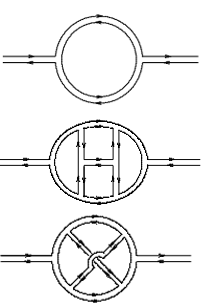
\includegraphics[width=0.4\textwidth]{Images/figurefull.png}
\caption{Double-line representation of a one-loop diagram for the gluon
propagator, four-loop diagram and a nonplanar diagram}
\label{fig:nonplanardiagrams}
\end{SCfigure}
This dependence on $N$ is also prescribed by the asymptotic-freedom formula
\begin{equation}
  g^2 = \frac{12\pi^2}{11N \textrm{ln}(\Lambda/\Lambda_{QCD})}
\end{equation}
of pure $SU(N)$ gauge theory.
\par Thus the contribution of the first diagram in \ref{fig:nonplanardiagrams}
is of order $\sim g^2N\sim 1$ in the large-$N$ limit.
We can think of the double lines as bounding a piece of a plane. These lines
represent a two-dimensional object. In mathematics these double-line graphs are
often called ribbon graphs or fatgraphs. They are deeply connected with Riemann
surfaces.
\subsubsection{Remark on the U(N) gauge group}
The double line representation of the diagrams holds, strictly speaking for the
$U(N)$ gauge group, whose generators
\begin{equation}
  T^A = (t^a, I/\sqrt{N}),\quad \mathrm{Tr}T^AT^B
  = \delta^{AB}\quad\boxed{A=1,\cdots,N^2}.
\end{equation}

obey the completeness condition

\begin{equation}
  \sum_{A=1}^{N^2}(T^A)^{ij}(T^A)^{kl}
  = \delta^{il}\delta^{kj}\quad\boxed{\mathrm{for}\quad U(N)}
\end{equation}
Elements of both $SU(N)$ and $U(N)$ can be represented in the form
\begin{equation}
  U = e^{iB}
\end{equation}
where $B$ is a general Hermitian matrix for $U(N)$ and a traceless Hermitian
matrix for $SU(N)$. The large-$N$ limit of both the $U(N)$ and $SU(N)$ groups
is the same.
\subsection{Planar and Nonplanar Graphs}
The double-line representation of perturbation theory diagrams is very
convenient to estimate their orders in $1/N$. Each three- or four-gluon vertex
contributes a factor of $g$ or $g^2$, respectively. Each closed index line
contributes a factor of $N$, while $g^2\sim 1/N$.
\subsubsection{'t Hooft topological expansion}
Let us consider a typical diagram for the gluon propagator as depicted in
\ref{fig:nonplanardiagrams} b). The sum over the $N$ indices is associated with
each of the four closed index lines, whose number is equal to the number of
loops. The contribution of this diagram is then $\sim g^8N^2\sim 1$.
\par Diagrams of this type, which can be drawn on a sheet of paper without
crossing any lines, are called \textit{planar diagrams}. For such diagrams, the
addition of a loop inevitably results in the addition of two three-gluon (or
one four-gluon) vertices. A planar diagram with $n_2$ loops has $n_2$ closed
index lines. It is of order
\begin{equation}
  n_2\mathrm{-loop}\;\mathrm{planar}\;\mathrm{diagram}\sim(g^2N)^{n_2}\sim 1,
\end{equation}
so that all planar diagrams survive in the large-$N$ limit. Let us now consider
a nonplanar diagram as the one depicted in \ref{fig:nonplanardiagrams} c). The
diagram has six three-gluon vertices but only one closed index line (although
it has 3 loops!). The order of this diagram is $\sim g^6N\sim 1/N^2$.
\par This nonplanar diagram can be drawn without line-crossing on a surface
with one handle (or hole) which in mathematics terms is called a torus of
a surface with genus one. A plane is then equivalent to a surface with genus
zero, which is in tern equivalent to a sphere. A general Riemanian surface with
$h$ holes has genus $h$.
\par The above evaluations of the order of the diagrams can now be described by
the single formula
\begin{equation}
  \mathrm{genus}-h\;\mathrm{diagram} \sim \left(\frac{1}{N^2}\right)^{\mathrm{genus}}.
  \label{eq:genusformula}
\end{equation}
The expansion in $1/N$ rearranges perturbation theory diagrams according to
their topology as demonstrated in 1974 by 't Hooft. It is referred to as the
topological expansion or the genus expansion. Only planar diagrams associated
with genus zero survive in the large-$N$ limit. The problem of summing the
planar graphs is complicated but simpler than that of summing all the graphs,
since the number of planar graphs with $n_0$ vertices grows geometrically at
large $n_0$:
\begin{equation}
  \sharp_p(n_0)\equiv\mathrm{\sharp\;of\;planar\;graphs}\sim\mathrm{const}^{n_0}
  \label{eq:numberofvertices}
\end{equation}
This was shown by Tuttle and Koplic, Beveu, Nussinov, while the total number of
graphs grows factorially with $n_0$. There is no dependence on the number of
external lines of a planar graphs in \eqref{eq:numberofvertices}, so it is
assumed to be much less than $n_0$.
\par There is a big difference between the planar diagrams and the ladder
diagrams which describe $e^+e^-$ elastic scattering in QED. For the ladder with
$n$ rungs, there are $n!$ ladder diagrams, but only one of them is planar. This
shows why the number of planar graphs is much smaller than the total number of
graphs, most of which are non-planar. Equation \eqref{eq:genusformula} holds,
strictly speaking, only for the gluon propagator, while the contribution of all
planar diagrams to a  connected $n$-point Green function is $\sim g^{n-2}$, 
which is its natural order in $1/N$. The three-gluon Green function is $\sim g$
, the four-gluon one is $\sim g^2$ and so on. The contributions of all 
planar diagrams are of the same order $\sim 1$ in the large-$N$ limit, 
independently of the number of external lines, for the Wilson loop average
\begin{multline}
  \big\langle\frac{1}{N}\mathrm{Tr}Pe^{ig\oint_\Gamma{\mathrm{d}x^\mu A_\mu
    (x)}}\big\rangle =\\
                     \sum_{n=0}^\infty i^n \oint_{\Gamma}\mathrm{d}x_1^{
      \mu_1}\int_{x_1}^{x_1}\mathrm{d}x_2^{\mu_2}\cdots\int_{x_1}^{x_{n-1}}\mathrm{d}x_n^{\mu_n}\mathrm{d}x_n^{\mu_n}G_{\mu_1\cdots\mu_n}^{(n)}(x_1,\cdots,x_n)
\end{multline}
where 
\begin{equation}
  G_{\mu_1\cdots\mu_n}^{(n)}(x_1,\cdots,x_n)\equiv\frac{g^n}{N}\langle\mathrm{Tr}\left[A_{\mu_1}(x_1)\cdots
    A_{\mu_n}(x_n)\right]\rangle.
    \label{eq:greeanfunctionlargen}
\end{equation}
The factor of $1/N$, which normalizes the trace, provides the natural
normalization. The ordering along a closed path implies cyclic-ordering in the
index space as depicted in Fig. \ref{fig:genericdoubleline} where we omit the
arrows for simplicity. This diagram has $n_0=10$ vertices, $n_1=12$ gluon
propagators, $n_2=4$ closed index lines, and $B=1$ boundaries.
\begin{figure}[h]
\begin{center}
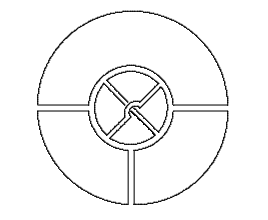
\includegraphics[width=0.3\textwidth]{Images/genericdoubleline.png}
\end{center}
\caption{Generic double-line index diagram}
\label{fig:genericdoubleline}
\end{figure}
The color indices of the external lines are contracted by the Kronecker delta
symbols (represented by the single lines) in a cyclic order. The extra factor
of $1/N$ arises from normalization. The order in $1/N$ of the diagram is $\sim
1/N^2$ in accord with \eqref{eq:genusformula}. Analogously, the color indices
in \eqref{eq:greeanfunctionlargen} are contracted in the cyclic order. The
delta-symbols, which contract the color indices, are depicted by the single
lines. They can be viewed as a boundary of the diagram. The actual size of
the boundary is not essential - it can be shrunk to a point. Then a bounded
piece of a plane will be topologically equivalent to a  sphere with a puncture.
We draw planar diagrams in a plane with an extended boundary (boundaries)
rather than in a sphere with a  puncture (punctures). The closed boundary is
associated with the trace over the color indices of the multi-point Green
function.
\par The boundary represents the Wilson loop - a trajectory of a heavy quark
in the fundamental representation.
\subsubsection{Topological expansion and quark loops}
It is easy to incorporate quarks in the topological expansion. A quark field
belongs to the fundamental representation of the gauge group $SU(N)$ and its
propagator is represented by a single line
\begin{equation}
  \langle\psi_i\bar{\psi}_j\rangle\propto\delta_{ij} =
  \feynmandiagram[small,inline=(a.base), horizontal = a to b]{
    a [particle=\(i\)]-- [fermion] b [particle=\(j\)];
};
\label{eq:quarkpropagator}
\end{equation}
The arrow indicates, as usual, the direction of propagation of a (complex)
field $\psi$. These arrows are often omitted for simplicity. The diagram for
the gluon propagator which involves one quark loop is  depicted in Fig
\ref{fig:gluonpropagator} a).
\begin{figure}[h]
\begin{center}
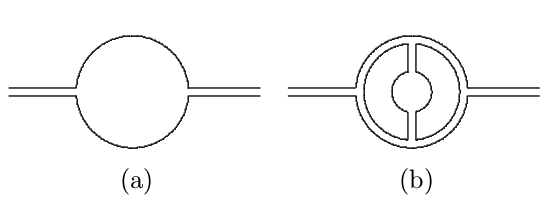
\includegraphics[width=0.6\textwidth]{Images/gluonquarkpropagator.png}
\end{center}
\caption{Diagrams for gluon propagator which involve quark loop}
\label{fig:gluonpropagator}
\end{figure}
It involves one quark loop and has no closed index lines so that its order is
$\sim g^2\sim 1/N$. The diagram in \ref{fig:gluonpropagator} b) is $\sim g^6N^2
\sim 1/N$ analogously. 
\par It is evident from this consideration that quark loops are not accompanied
by closed index lines. One should add a closed index line for each quark loop
in order for a given diagram with $L$ quark loops to have the same double-line 
representation as for pure gluon diagrams. Therefore, given
\eqref{eq:genusformula}, diagrams with $L$ quark loops are suppressed at large
$N$ by
\begin{equation}
  L\;\mathrm{quark\;loops}\sim \left(\frac{1}{N}\right)^{L+2*\mathrm{genus}}
  \label{eq:genusformulaquark}
\end{equation}
The single-line representation of the quark loops is  similar to that of the
Wilson loop. Such a diagram emerges in gluon corrections to the vacuum
expectation value of the quark operator:
\begin{equation}
  O = \frac{1}{N}\bar{\psi}\psi,
  \label{eq:quarkoperator}
\end{equation}
where the factor of $1/N$ is introduced to make it $\mathcal{O}(1)$ in the
large-$N$ limit. Therefore, the external boundary can be viewed as a single
line associated with valence quarks.
\subsubsection{The proof of topological expansion}
To prove \eqref{eq:genusformula} and it's quark counterpart
\eqref{eq:genusformulaquark}, let us consider a generic diagram in the index
space which has $n_0^{(3)}$ three-point vertices (either three-gluon
quark-gluon ones), $n_0^{(4)}$ four-gluon vertices, $n_1$ propagators (either
gluon or quark ones), $n_2$ closed index lines, $L$ virtual quark loops
and $B$ external boundaries. Its order in $1/N$ is
\begin{equation}
  \frac{1}{N^B}g^{n_0^{(3)}+2n_0^{(4)}}N^{n_2}\sim N^{n_2 - n_0^{(3)}/2
  - n_0^{(4)} - B}
  \label{eq:generaldiagram1n}
\end{equation}
as has already been explained. The extra factor of $1/N^2B$ arises from
the extra normalization factor of $1/N$ in operators associated with external
boundaries.
\par The number of propagators and vertices are related by
\begin{equation}
  2n_1 = 3n_0^{(3)} + 4n_0^{(4)},
\end{equation}
since three- and four-point vertices emit three or four propagators,
respectively, and each propagator connects two vertices. We then rewrite
the RHS of \eqref{eq:generaldiagram1n} as
\begin{equation}
  N^{n_2 - n_0^{(3)}/2 -n_0^{(4)} - B} = N^{n_2 - n_1 + n_0 -B},
  \label{eq:generaldiagram1nrhs}
\end{equation}
where $n_0 = n_0^{(3)} + n_0^{(4)} $ is the total number of vertices.
The exponent on the RHS of \eqref{eq:generaldiagram1nrhs} can be expressed
via the Euler characteristic $\chi$ of a given graph of genus $h$. An
appropriate Riemann surface, which is associated with a given graph,
is open and has $B+L$ boundaries. This surface can be closed by attaching
a cap to each boundary. The single lines then become double lines 
together with the lines  of the boundary of each cap. The number of faces for
a closed Riemann surface constructed in such a manner is $n_2+L+B$, while
the number of edges and vertices are $n_1$ and $n_0$, respectively. Euler's
theorem states that
\begin{equation}
\chi \equiv 2- 2h = n_2 + L + B -n_1+n_0.
\end{equation}
Therefore the RHS of \eqref{eq:generaldiagram1nrhs} can be rewritten as
\begin{equation}
  N^{n_2-n_1+n_0-B} = N^{2-2h-L-2B}.
\end{equation}
We have thus proven that the order in $1/N$ of a generic graph does
not depend on its order in the coupling constant and is completely 
expressed via the genus $h$ and the number of virtual quark loops $L$ and 
external boundaries $B$ by
\begin{equation}
  \mathrm{generic\;graph}\sim\left(\frac{1}{N}\right)^{2h+L+2(B-1)}
  \label{eq:genericgenusformula}  
\end{equation}
For $B=1$, we recover \eqref{eq:genusformula} and
\eqref{eq:genusformulaquark}.
\subsubsection{'t Hooft versus Veneziano limits}
In QCD there are several species or flavours of quarks. We denote the number
of flavours by $N_f$ and associate a Greek letter $\alpha$ or $\beta$ with a
flavour index of the quark field.
The quark propagator then has the Kronecker delta-symbol with respect to the
flavour indices in addition to \eqref{eq:quarkpropagator}
\begin{equation}
  \langle\psi^\alpha_i\bar{\psi^\beta_j}\rangle\propto
\delta^{\alpha\beta}\delta_{ij}
\end{equation}
Their contraction results in
\begin{equation}
  \sum_{\alpha=1}^{N_f}\delta_{\alpha\alpha} = N_f
\end{equation}
Therefore,  an extra factor of $N_f$ corresponds to each closed quark loop
for the $N_f$ flavours.
\par The limit when $N_f$ is fixed as $N\rightarrow\infty$ is called the 't
Hooft limit. Only valence quarks are then left (the quenched approximation). 
In order for a meson to decay into other mesons built out of quarks,
a quark-antiquark pair must be produced out of the vacuum. Consequently, the 
ratios of meson widths to their masses are
\begin{equation}
  \frac{\Gamma_{\mathrm{total}}}{M}\sim \frac{N_f}{N}
  \label{eq:widthmassratio}
\end{equation}
in the 't Hooft limit. The ratio on the LHS of \eqref{eq:widthmassratio} is 
10-15\% experimentally for the $\rho$-meson. The hope of solving QCD in the
't Hooft limit is the hope to describe QCD with this accuracy. An alternative
large-$N$ limit of QCD, when $N_f\sim N$ as $N\rightarrow\infty$ was proposed
by Veneziano in 1976. A general diagram with $L$ quark loops will contribute
\begin{equation}
L\;\mathrm{quark\;loops}\sim\left(\frac{N_f}{N}\right)^L\left(\frac{1}{N^2}\right)^\mathrm{genus},
\end{equation}
since each quark loop results in $N_f$.
\par The quark loops are not suppressed at large $N$ in the Veneziano limit
\begin{equation}
N_f\sim N\rightarrow\infty
\end{equation}
if the  diagram is planar. 
\par It is the Veneziano limit that is related to the hadronic topological
expansion in the dual-resonance models. In the Veneziano limit hadrons can have
finite widths according to \eqref{eq:widthmassratio}.
\subsection{Large-N factorization}
The vacuum expectation values of several colorless or white operators, which
are singlets with respect to the gauge group, factorize in the large-$N$ limit
of QCD (or other matrix models) as first was noticed by A.A. Migdal and
independently by E. Witten in late 1970's. The simplest gauge-invariant
operators in a pure $SU(N)$ gauge theory are the closed Wilson loops
\begin{equation}
  \Phi(C) = \frac{1}{N}\mathrm{Tr}Pe^{ig\oint_{C}\mathrm{d}z^\mu A_\mu(z)}.
\end{equation}
They obey the factorization property
\begin{equation}
  \langle\Phi(C_1)\cdots\Phi(C_n)\rangle
  = \langle\Phi(C_1)\rangle\cdots\langle\Phi(C_nC_n)\rangle
  + \mathcal{O}(N^{-2})
\end{equation}
The factorization implies a semiclassical nature of the large-$N$ limit of QCD
(a saddle point in the  path integral for certain variables). 
The factorization property also holds for gauge-invariant operators constructed
from quarks as in \eqref{eq:quarkoperator}. For the case of several flavours
$N_f$, we normalize these quark operators by
\begin{equation}
O_\Gamma = \frac{1}{N_f N}\bar{\Psi}\Gamma\psi
\end{equation}
Here, $\Gamma$ denotes one of the combination of the $\gamma$-matrices:
\begin{equation}
  \Gamma = I,\gamma_5,\gamma_mu,i\gamma_\mu\gamma_5,\sum_{\mu\nu}
  = \frac{1}{2i}\left[\gamma_\mu,\gamma_\nu\right],\cdots.
\end{equation}
The factorization of the gauge-invariant quark operators hold both in the 
't Hooft and Veneziano limits:
\begin{equation}
\langle O_{\Gamma_1}\cdots O_{\Gamma_n}\rangle
= \langle O_{\Gamma_1}\rangle\cdots\langle O_{\Gamma_n}\rangle+
\mathcal{O}(1/(N_fN)).
\label{eq:factorizationproperty}
\end{equation}
The nonfactorized part, which is associated with connected diagrams is $\sim
1/N$ in the 't Hooft limit. This leads, in particular, to the coupling constant 
of meson-meson interaction of order $1/N$. The Veneziano limit it analogous to
pure Yang-Mills.
\par The factorization can be seen (at all orders of perturbation theory) form
\eqref{eq:genericgenusformula} for the contribution of a generic connected
graph of genus $h$ with $B$ external boundaries which are precisely associated 
with the Wilson loops (or the quark operators). The diagrams with gluon lines
emitted and absorbed by the same operator are products of diagrams having
only one boundary. Their contribution is of order one. The diagrams with gluon
lines emitted and absorbed by two different operators have two boundaries.
This proves the factorization property \eqref{eq:factorizationproperty} at all
orders of perturbation theory.
\par The large-$N$ factorization can also be verified beyond perturbation
theory at all orders  of the strong-coupling expansion of the $SU(N)$ lattice
gauge theory. A non-perturbative proof of the factorization was given using 
quantum equations of motion (the loop equations).
\subsection{Conclusion}
We have considered in this section the basic features of the methods for
nonperturbative studies of gauge theories, which were developed in the
second half of 1970's- early 1980's. Their contemporary applications in
high-energy physics are extremely broad: from the scattering of particles at
very high energies of the attempts of constructing a unified theory of all
interactions, including gravity.
